\graphicspath{{content/chapters/3_literature/figures/}}
\chapter{Literature Review}
\label{sec:literature_review}

This chapter presents an overview of deep learning methods for speech enhancement, with a focus on the autoencoder architecture. It outlines the basic principles, training process, and recent advancements in this field, while also introducing the performance metrics used to evaluate enhancement models.


\section{Neural Networks}
\label{sec:neural_networks}

Machine learning models, particularly neural networks, have been widely adopted for noise cancellation. Neural networks, inspired by biological neurons in the human brain, are composed of layers of interconnected processing units known as \textit{neurons}. Each artificial neuron receives multiple inputs, performs a weighted summation, applies a bias, and passes the result through an activation function to produce its output.

This structure draws direct inspiration from the way biological neurons function—where dendrites receive signals, the cell body processes them, and the axon transmits the signal to the next neuron. Figure~\ref{fig:neuron_vs_ann} illustrates this analogy.

\begin{figure}[H]
    \centering
    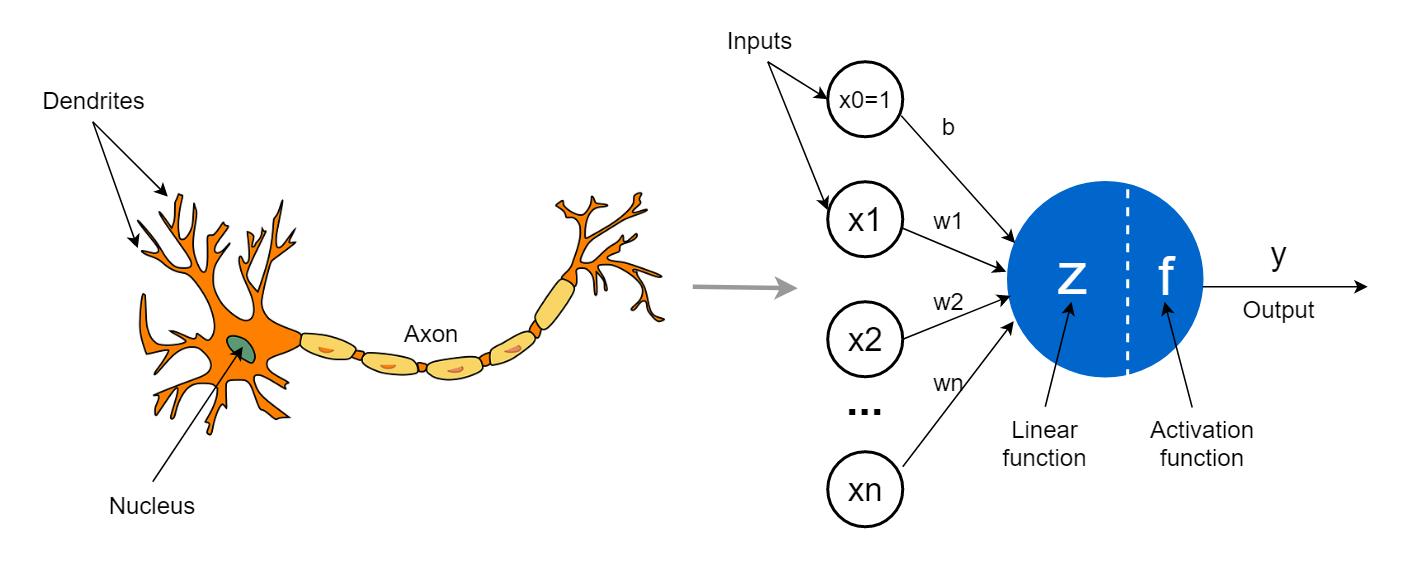
\includegraphics[width=0.75\textwidth]{neuron_vs_ann.png}
    \caption{Biological neuron vs. Artificial neuron structure.\cite{ghosh2020perceptron}}
    \label{fig:neuron_vs_ann}
\end{figure}

A typical neural network for noise cancellation consists of the following components:
\begin{itemize}
    \item \textbf{Input layer:} Receives the noisy speech signal (e.g., a time-domain waveform or its spectrogram).
    \item \textbf{Hidden layers:} Perform nonlinear transformations to extract key features and patterns from the input. These layers may include convolutional, recurrent, or fully connected neurons depending on the network architecture.
    \item \textbf{Output layer:} Produces the denoised speech signal by mapping the learned features back to the clean signal domain.
\end{itemize}

The network is trained using pairs of clean and noisy audio samples. It gradually learns to reduce the difference between its predicted output and the actual clean signal. Once trained, the model can take in new noisy speech and output a cleaner version. This learning-based approach allows neural networks to adapt to complex noise patterns, often performing better than traditional signal processing methods in real-world situations.

\section{Machine Learning}
\label{sec:machine_learning}

Machine learning (ML) is a subset of artificial intelligence (AI) that focuses on the development of algorithms and statistical models that enable computers to perform specific tasks without explicit instructions. Instead, these systems learn from data, identifying patterns and making decisions based on their experiences. In the context of speech enhancement, ML has provided basis for advanced with specialised neural network architectures tailored for this task. One of the most widely adopted structures is the \textit{autoencoder}, a neural network designed to reconstruct its input through a compressed internal representation \cite{azarang2020review}.

\begin{figure}[h]
    \centering
    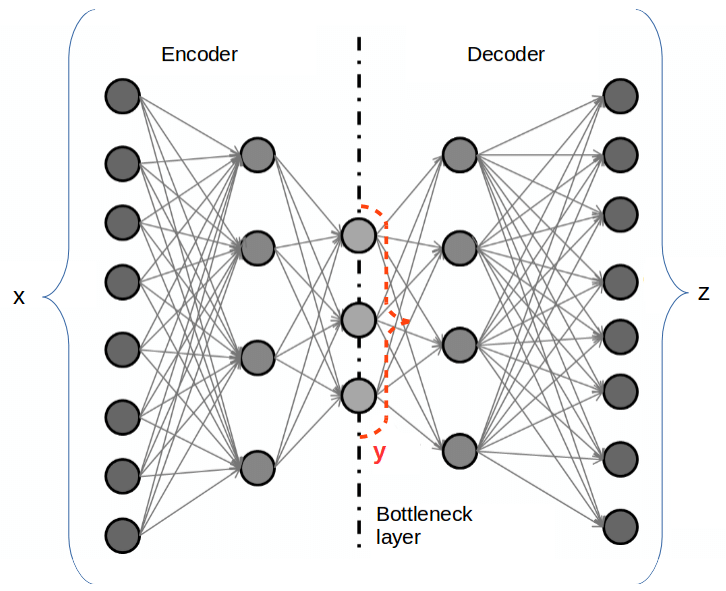
\includegraphics[width=0.5\textwidth,keepaspectratio]{autoencoder.png}
    \caption{\label{fig:autoencoder} Block diagram of an autoencoder architecture \cite{vachhani2017dae}.}
\end{figure}

An autoencoder typically comprises two main components: the encoder and the decoder. The encoder compresses the input data \(x\) into a lower-dimensional latent representation. This component often consists of multiple layers—such as convolutional, pooling, and fully connected layers—each applying a set of learnable parameters to extract increasingly abstract features. The goal of the encoder is to distil essential information from the input while discarding noise and irrelevant variations.

Between the encoder and decoder lies the bottleneck layer. This layer enforces compression by limiting the dimensionality of the latent representation, encouraging the network to retain only the most salient features. As a result, the model learns a compact representation that captures the structure of clean speech while ignoring extraneous noise.

The decoder then reconstructs the output \(y\) from this compressed form, typically using upsampling, deconvolutional, and dense layers arranged in a mirrored architecture relative to the encoder. Its objective is to restore the original input with minimal error, ideally recovering a clean version of the speech signal from its noisy counterpart.

A critical question arises: how does the autoencoder learn to denoise during training? The key lies in the use of paired datasets consisting of noisy and clean speech samples. During training, the model receives the noisy signal as input and is optimised to minimise the difference between its output and the clean reference. This difference is quantified using a loss function, most commonly the Mean Squared Error (MSE) or Mean Absolute Error (MAE), which measures the average discrepancy between the reconstructed and target signals.

\begin{figure}[h]
    \centering
    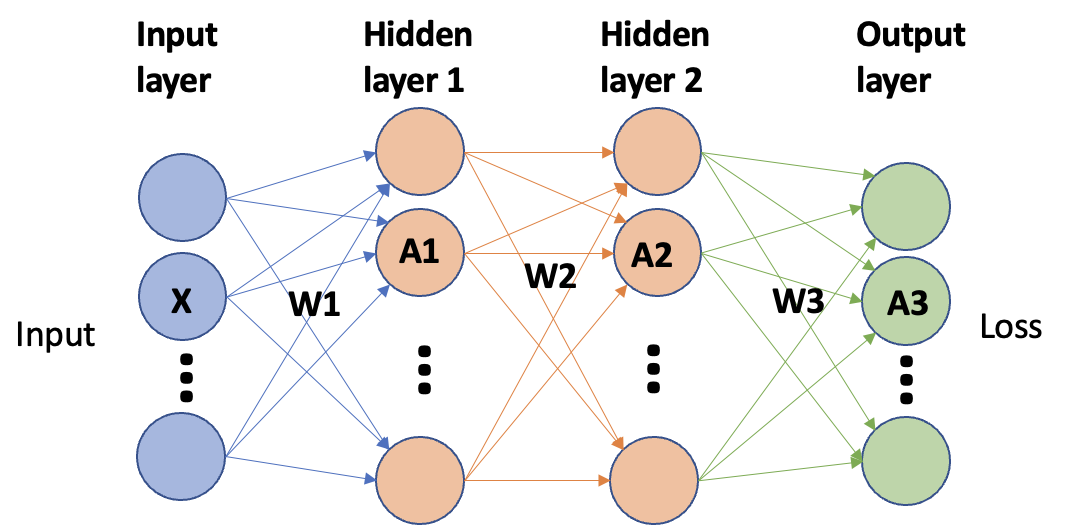
\includegraphics[width=0.5\textwidth,keepaspectratio]{weigths.png}
    \caption{\label{fig:weigths} Loss and weight update process in an autoencoder \cite{epoch2021}.}
\end{figure}

The training process proceeds iteratively. A forward pass propagates the noisy input through the network to produce an output. This output is compared with the clean target using the loss function. The error is then propagated backwards through the network via backpropagation to calculate gradients. These gradients are used to update the model’s weights and biases using an optimisation algorithm, such as Stochastic Gradient Descent (SGD) or Adam. This loop is repeated over many epochs until the model converges to a configuration that minimises reconstruction error.

Recent advancements continue to refine both model architectures and training strategies in deep learning for speech enhancement. New variations introduce more robust designs capable of generalising to a broader range of noise conditions. One notable example is a study that proposed a residual-attention Gated Linear Unit (GLU) structure for end-to-end (E2E) speech enhancement \cite{kim2024residual}. The model demonstrated superior performance over state-of-the-art (SOTA) systems such as FAIR-Denoiser and CleanUNet across a range of signal-to-noise ratios (SNR) from 0 to 15 dB.

Moreover, the evaluation metrics adopted in these studies—such as SNR, PESQ, STOI, and MSE—are integral to assessing model performance and will also be employed in this project to benchmark classical and deep learning approaches. These metrics will be explored further in Chapter~\ref{chp:evaluation}.
